Fuel station skimming is both increasingly widespread and difficult to observe
due to the number of possible targets.
%
For example, in 2017 the Arizona Department of Weights and Measures (AZWM)
found 57 skimmers; so far in 2018 they have found over 100 skimmers (175\%
increase).
%
In Arizona, there are approximately 2,400 fuel stations, and so far in 2018
AZWM inspectors have only found skimmers at 66 fuel stations (2.8\%).
%
% Duplicate statement to paragraph above
% Finding skimmers is like finding a needle in a haystack.
%
In San Diego County there are 875 fuel stations, and so far in 2018 inspectors
from the U.S. Secret Service (USSS) have only found skimmers at 12 fuel stations
(1.4\%).

Adding to the challenge is the fact that criminals distribute their skimmer
installs over a large area, covering both urban and rural fuel stations.
%
In San Diego County, the shortest path distance between the 12 fuel stations
that were found to have skimmers is 133 miles; that is over three hours of
drive time.
%
In Arizona, the shortest path distance between the 66 fuel stations that were
found to have skimmers is is 637 miles, that is 14.5 hours of drive time.

% Additionally, they passively tap into the existing card reader and keypad
% electronics; they defeat the most advanced skimmer detection tools that look
% for extra card reading hardware~\cite{skimreaper2018}.

Unfortunately, until this work, the only proven method of determining if a fuel
station is affected is to wait for fraud alerts from banks, and to react to
often flaky consumer complaints.
%
Inspectors in several states (i.e., Arizona) have such a large skimming problem
in their jurisdictions that they have even resorted to costly periodic manual
inspections of every dispenser in every fuel station.

For every fuel station that an inspector visits and does not find a skimmer,
this gives the criminals more lead time to install skimmers.
%
This is important because fuel stations tend to have repeat skimming attempts.
Of the 66 fuel stations hit with skimmers in Arizona, 20 were reported to have
skimmers once more within the year.
%
Even within the scope of our in-depth study we saw repeated skimming at the
same fuel station: we discovered skimmers on all but one dispenser at a fuel
station in Pacific Beach, CA, and after law enforcement recovered them, they
were installed on four dispensers two months later.
%


\begin{comment}
    We can quantify exactly how much time inspectors spend on stations that did not
    have skimmers.
    %
    Surveying the inspection reports in 2018, we found that they performed 867
    inspections of fuel stations---of which only 86 (5\%) resulted in newly
    discovered skimmers.
    \begin{figure}
        \centering
        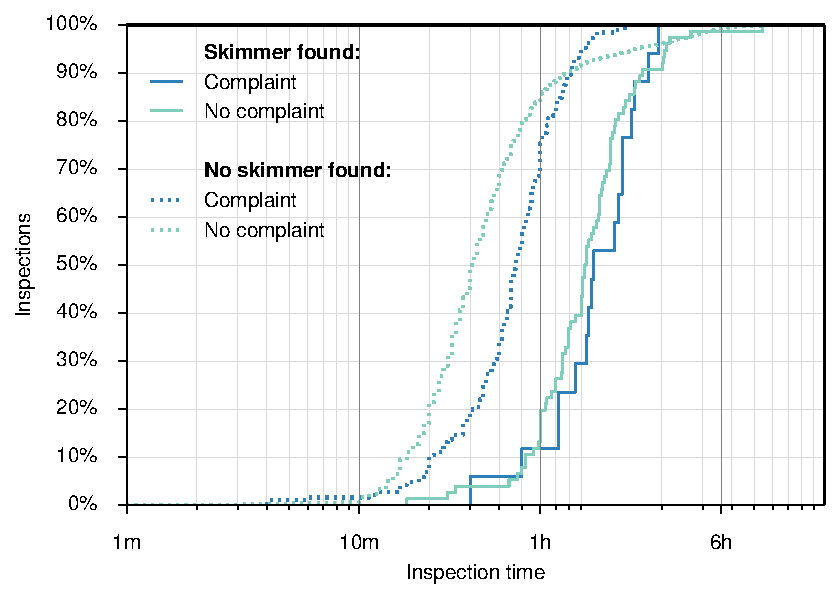
\includegraphics[width=\linewidth]{plots/arizona_analysis_all.pdf}
        \caption{
        \label{fig:cdf_arizona_timetaken}
        Half of the unsuccessful manual inspections for skimmers took over half an hour to search the dispensers.
        }
    \end{figure}

    We also can quantify how much time inspectors spend on fruitless inspections.
    %
    Along with reporting if a skimmer was found or not, the Arizona inspection
    reports also contain the time the inspection started and ended, allowing us to determine how long each inspection took.
    %
    Figure \ref{fig:cdf_arizona_timetaken} shows the distribution of durations for inspections that found skimmers and inspections that did not.
    %
    The median time taken for an unsuccessful inspection is 32 minutes, most
    inspections were an hour or less, and the longest inspection took over three
    hours. \noteby{KL}{Update this text.}
    %
    In total, 168 person-hours, or about a month of full-time (40 hours/week) labor
    was spent performing unsuccessful inspections over the course of four months.
    %
    Note that this is a conservative estimate because it does not include
    transportation time, only the time spent opening and searching fuel dispensers.
    %
    Given limited agency resources, a skimmer may be in place for months before it is found by a random inspection.
\end{comment}


xxx

As of the current year, a criminal can still use the track 1 and 2 data off of a frauded card to purchase products at
some stores for resale at lower than the purchase price. \cite{cardingGeneralGuide, howToSucceedInStore}
%
The range of products purchased varies widely, including everything from gasoline\footnote{This has the advantage of
looking innocuous to the card issuer and card holder, but has the disadvantage of managing a flammable liquid and
visiting the station in a car with covered plates.} \cite{krebsbladder} to online poker
accounts \cite{cardingPokerstars} to gaming stations and Iphones \cite{cardingBuyStuff}.
%
However, gas cards may only be used for fuel purchases.
%
Due to the nature of this form of fraud, the value attained from each card by the criminal varies by individual choice
and a multifactor system incorporating the ability of the card issuer to detect the fraudulent purchase, the criminal's
choice of the product to buy, and the amount of money in the card's account. \cite{viceInterviewWithCarder}
%
Cheaper cards typically have an upper purchase limit of \$500, with business and signature cards having a limit of
thousands of dollars.~\cite{cardingGeneralGuide}
%
The criminal will resell the stolen goods, most likely at a loss, so we have given this form of fraud a range
between \$300 and \$500 dollars per day for classic cards \cite{cardingNewbieGuide, viceInterviewWithCarder}.
%
The value the criminal gets from the purchase is also less than the market value of the good; for example, one forum
post is reselling Iphone X's for \$400 dollars rather than the \$769 as of time of writing. \cite{iphoneXSale}





\note{xxx KL xxx}


In the following section we will attempt to quantify the impact of installed skimmers through a direct study of online
skimming forums, a literature review, and a memory dump of 10 skimmers given to us by government officials. We will be
focused primarily on the amount of card data that a criminal can pull from a skimmer over an approximately 24 to 48
hour time period, as well as the amount of money that can be attained from a stolen debit or credit card. Results
are summarised in Table \ref{tab:skim-cost-breakdown}

\begin{table*}
    \centering\small
    \begin{tabular}{lcc}
    \toprule
    \colname{Card Value Scheme} & \colname{Value} & \colname{Source} \\
    \midrule
    \textbf{Direct Data Sale} \\
    \quad Debit, Credit \/w pin Standard & \$110, \$120 & Online sale sites and forums \cite{legitshop, dumpsPrtShip} \\
    \quad Debit, Credit \/w pin Business, Premium & \$220 & Online sale sites and forums \cite{legitshop, dumpsPrtShip} \\
    \quad Classic\/Standard & 10, 20, 25 USD& Online sale sites and forums \cite{meccadumps,legitshop, sellcvv,dumpsto, dumpsPrtShip}\\
    \quad Gold\/Platinum & 15, 20, 25 USD & Online sale sites and forums \cite{meccadumps,legitshop, sellcvv,dumpsto, dumpsPrtShip}\\
    \quad Signature\/Business & 40,60 USD & Online sale sites and forums \cite{meccadumps,legitshop, sellcvv,dumpsto, dumpsPrtShip}\\
    \quad Purchasing\/Corporate\/World & 30, 40 USD & Online sale sites and forums \cite{meccadumps,legitshop, sellcvv,dumpsto, dumpsPrtShip}\\
    \quad Amex & 6, 10 USD & Online sale sites and forums \cite{meccadumps,legitshop, sellcvv,dumpsto, dumpsPrtShip}\\
    \quad Discover & 10, 20 USD & Online sale sites and forums (I have more sites if needed )\cite{meccadumps,legitshop, sellcvv,dumpsto, dumpsPrtShip}\\
    \textbf{ATM} \\
    \quad Debit/Credit Typical Draw Limit & \$500, \$1,000, \$2,000 & Bank FAQs, various online blogs \cite{boaWithdraw, santandWithdraw, debitCapsForEachBank} \\
    \quad Debit/Credit Premium (and Custom) Draw Limit & \$2,500, \$4,000 & Bank FAQs \cite{santandWithdraw, boaWithdraw} \\
    \textbf{Product Resale} \\
    \quad General Advice (Standard Cards) & \$500, \$800 & various online tutorials, interviews \cite{cardingNewbieGuide, howToSucceedInStore, viceInterviewWithCarder} \\
    \quad General Advice (Standard Cards) & \$400-\$600 & anecdotes on carding forums \cite{makingFirstMoney} \\
    \quad General Advice (Premium Cards) & \$1,000 h & anecdotes from tutorials \cite{cardingNewbieGuide} \\
    \quad Iphones & \$400 & Carding Resale Sites \cite{iphoneXSale} \\
    \quad Macbooks & \$1000 & Carding Resale Sites \cite{iphoneXSale} \\
    \quad Playstations & \$210 & Carding Resale Sites \cite{ps4Sale, viceInterviewWithCarder} \\
    \quad Gasoline & \$75, \$125 & Kerbs article \cite{krebsbladder, nacsHoldReport} \\
    \quad Online Poker & \$150 & Online Forum Suggestion \cite{poker150Suggest} \\
    \textbf{Damage} \\
    \quad Credit (to Consumer) & max. \$50 & U.S. Code 1643. \cite{cornellliability} \\
    \quad Debit (to Consumer) & \$500 (60 days) &  U.S. Code 1693g \cite{1693g} \\
    \quad Credit and Debit (to Bank and Merchant) & \$902 & Dept. of Justice average loss \cite{harrell2017} \\
    \quad Credit and Debit (to Bank and Merchant) & \$500 & Arizona Dept. of Weights and Measures \cite{arizonareport} \\
    \quad Credit and Debit (to Bank and Merchant) & \$650 & National Cash Register (NCR) \cite{rippleshot} \\
    %    \colname{Card Scheme} &  \multicolumn{3}{c}{\colname{Debit}} & \multicolumn{3}{c}{\colname{Credit}} \\
    %    \cmidrule(lr){2-4} \cmidrule(lr){5-7}
    %    \colname{Data Available} & \colname{pin} & \colname{zip} & \colname{no pin / zip} & \colname{pin} & \colname{zip} & \colname{no pin/zip} \\
    %    \midrule
    %    cash value wholesale & \multicolumn{1}{|c|}{\$110 - \$220} & \multicolumn{1}{c|}{\$5 - \$60} & \multicolumn{1}{c|}{\$10} & \multicolumn{1}{c|}{\$110} & \multicolumn{1}{c|}{\$10 - \$60}& \multicolumn{1}{c}{\$5 - \$10}\\
    %    \hline
    %    ``classic'' cash value & \multicolumn{1}{|c|}{\$500+ (ATM)} & \multicolumn{2}{c|}{\$300 - \$500 }& \multicolumn{1}{c|}{\$500+ (ATM)} & \multicolumn{2}{c|}{\$300 - \$500 } \\
    %    \hline
    %    ``business / platinum'' cash value & \multicolumn{1}{|c|}{\$1000+ (ATM)} & \multicolumn{5}{c|}{\$500+} \\
    %    \hline
    %    average tracks per pull & \multicolumn{1}{|c|}{7.9} & \multicolumn{1}{c|}{1.5} & \multicolumn{1}{c|}{1.1}& \multicolumn{1}{c|}{0.6}&  \multicolumn{1}{c}{7.1} & \multicolumn{1}{|c}{1.5} \\
    %    \hline
    %    Min. value per skimmer per pull per day & \multicolumn{1}{|c|}{\$4,000} & \multicolumn{1}{c|}{\$600} & \multicolumn{1}{c|}{\$440}& \multicolumn{1}{c|}{\$300} &  \multicolumn{1}{c}{\$2,840} & \multicolumn{1}{|c}{1.5} \\
    %    \hline
    %    Approx. total value per pull per day & TODO once numbers solid \\
    %    Number of skimmers stopped by Bluetana & 39 \\
    %    Fraud prevented by bluetana assuming crimnals reinstalled skimmers the next day & X \\
    % The cards can be reused each day, or if sold on an online forum, it can be sold to multiple people the criminal
    % can use the cards to buy multiple playstations, withdraw from ATMs, etc..
    % Sites (many are temporary): https://meccadumps.net legitshop.org dumps.to sellcvvdumps.shop
    %    Debit with ZIP and PIN & \$100 - \$200  \\
    %    Out-of-pocket loss & \$902 \\
    %    Worth to criminal & \$500 \\
    %    Portion of fraud borne to bank  & \$500 - \$1000 \\
    %    Portion of fraud borne to individual  & \$50 - \$500 \\
    % Credit with ZIP, track 1 and 2 & \$25 - \$35 \\
    % Credit with ZIP and track 2 & \$15 - \$25 \\
    % Debit with no PIN & \$7 - \$40  \\
    % Debit (premium) with ZIP and PIN & \$200 - \$500  \\
    % % https://www.justice.gov/usao-edca/pr/leader-target-department-store-credit-card-fraud-scheme-sentenced-65-years-prison
    % Card worth to criminal (DOJ Estimate) & \$500  \\
    % Card worth to criminal (hearsay) & \$498, \$900  \\
    % % Nilson Report 2016, Javelin, Various Slides
    % Fraud cost to retailer (Reported) & \$400  \\
    % Fraud cost to retailer (Law Enforcement) & \$0  \\
    % Fraud cost to individual (Credit) & \$0 - \$50 \\
    % Fraud cost to individual (Debit) & \$50 - 500 \\
    \bottomrule
\end{tabular}
    \caption{Estimate of the amount of cash a criminal can make per skimmer per day.}
    \label{tab:skim-cost-breakdown}
\end{table*}





%Various idiosyncrasies occur: corruption and partially failed installations are common.
%%
%Out of the 251 records, X were completely corrupted, leaving XX in tact.
%%
%Y failed to record track one data properly but retained correct track two data. Z recorded track one properly and not
%track two.
%%
%Z were missing a pin number or zip.
%%%
%The hardware engineering of skimmers is often uniform and professionally done, installation is not undertaken with
%the same care.
%%
%YY cases of failed track one data reads were due to an incomplete installation of one skimmer.
%%
%Orthogonally, the nature of the magnetic strip oftentimes prevents complete corruption; the removal of these ``bad
%install'' records leaves YYY card records ``saved by the duplication of account number across two tracks.
%
%For those records which were not completely corrected, we were able to determine duplicate card swipes in X of the
%records.
%%
%This is most likely due to mistyped pins or complications caused by the skimmer's interference, as none of the duplicate
%records were seen separated by a transaction using another card.
%
%Of the remaining records, the card BIN/IIN numbers revealed statistics on debit and credit card ratios.
%%
%These results are recorded in table \ref{tab:skim-dump-results}.
%%
%The estimates currently given for the number of cards per skimmer seem to be correct ... \noteby{MB}{Further analysis
%of the table.}
%%
%Only X\% of the cards could be concretely classified as gas cards given out to a fleet vehicle.

\subsection{Economic Impact}

Next we will look at how criminals gain money through skimming, as well as the collateral economic damage created
by the fraud economy orbiting fuel sales in the the United States.

\subsubsection{Fraud Overview}

Card fraud is, at best, a pareto efficient zero-sum game, wherein the amount the criminal gains via skimming is
equivalent to the amount lost by other parties.
%
There are numerous levels of management and repair costs associated with card fraud, and this leads to inefficiency.
%
The Nilson Report, a payment industry surveyor, reported in 2016 that the total cost of card fraud to card issuers
was 15.72 billion, to merchants 5.9 billion, and to ATM acquirers 217.4 million~\cite{nilsonreport2016}.
%
Javelin research, a reporting entity on identity fraud, has reported that the number of identity fraud cases was 15.4
million in 2016 with \$16 billion in damages.~\cite{javelinstudy}
%
These numbers include losses due to online fraud and non-skimmer criminal activity, but demonstrate the impact that
fraud has on the economy annually.
%
The goal of this work is to reduce the negative impacts of card skimming and improve the overall efficiency of payment
transactions.


\subsubsection{Criminal Cashout}

Getting a clear understanding of the daily skimmer ``catch'' is straight-forward, but the quantification of the
economic cost is not.
%
This is partially because the criminal can ``cash out'' multiple times from a given card if the fraud is not noticed.
%
Difficulty also manifests due to the variety of ways money can be made from card data.

\paragraph{ATM Withdrawals}
If the criminal attains a debit card with a pin code, the criminal may use a ``blank'' to create a duplicate card for
use at ATMs to withdraw money.
%
This method has a fraud cap each day of around \$500 in the typical case, but can be up to \$9,000 depending on the
card type. \cite{boaWithdrawalLimit, debitCapsForEachBank}
%
Note that in the case where a victim has activated the pin feature of their credit card, the criminal may use this to
perform a cash advance (potentially) up to the card's credit limit. \cite{boaCashAdvanceFaq}



%
%Figure~\ref{fig:criminal_showing_off_cash} is taken from a screenshot posted to one of the card selling forums we
%investigated, and is representative of reports we have received from law enforcement.
%


%\begin{figure}
%    \centering
%    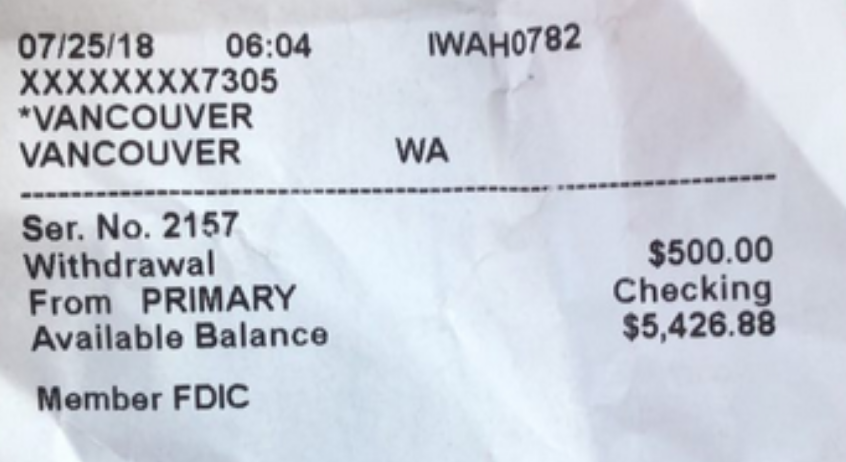
\includegraphics[width=\linewidth]{fig/criminal_showing_off_cash.png}
%    \caption{
%    The amount typically withdrawn from a victims bank account is the ATM cutoff amount.
%    }
%    \label{fig:criminal_showing_off_cash}
%\end{figure}

\paragraph{Product Purchase}

As of the current year, a criminal can still use the track 1 and 2 data off of a frauded card to purchase products at
some stores for resale at lower than the purchase price. \cite{cardingGeneralGuide, howToSucceedInStore}
%
The range of products purchased varies widely, including everything from gasoline\footnote{This has the advantage of
looking innocuous to the card issuer and card holder, but has the disadvantage of managing a flammable liquid and
visiting the station in a car with covered plates.} \cite{krebsbladder} to online poker
accounts \cite{cardingPokerstars} to gaming stations and Iphones \cite{cardingBuyStuff}.
%
However, gas cards may only be used for fuel purchases.
%
Due to the nature of this form of fraud, the value attained from each card by the criminal varies by individual choice
and a multifactor system incorporating the ability of the card issuer to detect the fraudulent purchase, the criminal's
choice of the product to buy, and the amount of money in the card's account. \cite{viceInterviewWithCarder}
%
Cheaper cards typically have an upper purchase limit of \$500, with business and signature cards having a limit of
thousands of dollars.~\cite{cardingGeneralGuide}
%
The criminal will resell the stolen goods, most likely at a loss, so we have given this form of fraud a range
between \$300 and \$500 dollars per day for classic cards \cite{cardingNewbieGuide, viceInterviewWithCarder}.
%
The value the criminal gets from the purchase is also less than the market value of the good; for example, one forum
post is reselling Iphone X's for \$400 dollars rather than the \$769 as of time of writing. \cite{iphoneXSale}

\paragraph{Online Wholesale}

% https://deluxedumps.com/shop
% https://fridaydumps24.com/shop
Another route of sale does not involve manufacturing a counterfeit card at all.
%
Various black market sites offer "dumps", which constitute of magnetic stripe information (pin number optional)
from cards. \cite{meccadumps,legitshop, sellcvv,dumpsto, dumpsPrtShip}
%
An alternative, "CC", or "fullz", contain more information (such as the victim's address), but these cards are likely
the result of phishing and breaches rather than skimming.
%
There is a wide variation in card prices depending on whether a refund is offered in the case of a non-working card,
the credit cap on the card, and whether the card has a known pin.
%
For debit and credit cards without PIN, there is a large range of prices, from \$5 for low quality cards or cards with
little money on them, to \$500 dollars or more for Mastercard Platinum, BestBuy, and Business class
cards. \cite{meccadumps, dumpsto, dumpsPrtShip, mrwhite}
%
Debit cards with PIN do have a relatively stable price: on the range of \$100 to \$220 dollars. \cite{sellcvv, legitshop}
%
Discussions with the US Attorney general's office and government inspectors have suggested that criminals
prefer to take advantage of skimmed cards themselves rather than sell them online.


\subsubsection{Collateral Damage}

Under federal law, the most a victim may be charged for credit card fraud is \$50. \cite{cornellliability}
%
There is potentially a much higher cost to the consumer associated with debit card fraud, defined by the
Federal Electronic Fund Transfer Act.
%
There is \$0 liability if the fraud is reported before the card is used, \$50 if it is reported within two days,
up to \$500 dollars liability if fraud is not reported within sixty days, and an unlimited amount if more
than sixty days pass. \cite{1693g}

Surveys done by the US Department of Justice have determined the out-of-pocket collateral cost of skimming to be around
\$902, but estimates vary. \cite{harrell2017}
%
Our own government contacts have estimated the range of cost to the bank and merchant to be between \$500 and \$1000
dollars.
%
Estimates done on the cost by the Arizona Department of Weights and Measures and others have placed the cost to the
bank and retailer at around \$500.~\cite{arizonareport, rippleshot}
%
If the fraud is reported within a reasonable time frame, it is assumed that the bank or retailer will cover the cost of
the fraud and restore the balance of the victim through various insurance policies.
%
Doing so will incur additional management costs: running call centers, mailing replacement cards, and staffing bank
branches.

\subsubsection{The Cost of Skimming}

We have seen that criminals can make, conservatively, around four to fifteen thousand dollars per day from a single
skimmer until the fraud is noticed and reported.
%
In a conservative estimate, Bluetana's removal of 38 skimmers has therefore prevented a minimum of
152 thousand dollars of fraud.

%The amount of money involved has been enough to sustain a skimming micro-economy; many ``.onion'' domains, facebook
%pages, and blogspot stores offer their own brands of skimmers for approximately \$400 dollars and pyramid schemes
%with payment plans \cite{blogspotSaleSite,skimmerFacebookPage}

However, this ``skimmer'' economy is built around market inefficiencies.
%
The downside to this is that any money the criminal uses must eventually be restored by the merchant or the bank plus
administrative costs.
%
In many cases, the criminal makes less off of the card than the amount frauded.
%
If a criminal buys a PlayStation 4 for \$500 dollars and sells it to a pawn shop for \$300, and the merchant must
restore the entire \$500 dollar cost back to the victim's account, then this action has created a loss of \$200
dollars in utility.

%\subsection{Vulnerable Fuel Dispensers}
%\label{subsec:vulnerable-fuel-dispensers}
%\noteby{KL}{This is the Streetview study. Not sure what to do with it yet.}
%
%In order to evaluate the current state of pump security, we estimated the
%proportion of pumps that are vulnerable to universal key attacks by surveying
%fuel dispenser deployments. \noteby{MB}{We've also done this for a random
%sampling of pumps across the country. We should also make the transition into
%this point from the prior paragraph smoother}
%%
%Specifically, we used Google Street View to manually classify the fuel dispenser
%make/model of the 875 gas stations in in one of the ten largest cities in the
%United States.
%%
%We found that 31\% (271) of the stations were using a popular model of
%dispenser that has a universal key.
%%
%We found that the vulnerable dispensers are installed in both the urban and
%suburban areas, although the concentration is in rural areas. \noteby{MB}{If you say this, gimme the numbers.}
%%
%Although there are fewer vulnerable pumps in urban areas, these locations are
%still targeted: we discovered one urban gas station compromised by skimmers on
%seven dispensers---all but one in the station.
%}}}

